\mbox{$\displaystyle \frac{1}{4}$\,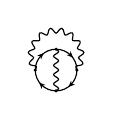
\begin{tikzpicture}[x=0.340cm, y=0.340cm, line width=0.420pt, baseline={([yshift=-0.6ex]0,0)}]
  \draw (-0.778,0.000) arc[start angle=180.000, end angle=90.000, radius=0.778];
  \fill (-0.466,0.634) -- (-0.707,0.538) -- (-0.580,0.520) -- (-0.562,0.393) -- cycle;
  \draw (0.000,0.778) arc[start angle=90.000, end angle=0.000, radius=0.778];
  \fill (0.634,0.466) -- (0.538,0.707) -- (0.520,0.580) -- (0.393,0.562) -- cycle;
  \draw (0.000,-0.778) arc[start angle=270.000, end angle=180.000, radius=0.778];
  \fill (-0.634,-0.466) -- (-0.538,-0.707) -- (-0.520,-0.580) -- (-0.393,-0.562) -- cycle;
  \draw (0.778,0.000) arc[start angle=0.000, end angle=-90.000, radius=0.778];
  \fill (0.466,-0.634) -- (0.707,-0.538) -- (0.580,-0.520) -- (0.562,-0.393) -- cycle;
  \draw plot[smooth, tension=0.7] coordinates {(0.000,0.778) (0.066,0.735) (0.093,0.691) (0.066,0.648) (0.000,0.605) (-0.066,0.562) (-0.093,0.519) (-0.066,0.475) (0.000,0.432) (0.066,0.389) (0.093,0.346) (0.066,0.302) (0.000,0.259) (-0.066,0.216) (-0.093,0.173) (-0.066,0.130) (0.000,0.086) (0.066,0.043) (0.093,0.000) (0.066,-0.043) (0.000,-0.086) (-0.066,-0.130) (-0.093,-0.173) (-0.066,-0.216) (0.000,-0.259) (0.066,-0.302) (0.093,-0.346) (0.066,-0.389) (0.000,-0.432) (-0.066,-0.475) (-0.093,-0.519) (-0.066,-0.562) (0.000,-0.605) (0.066,-0.648) (0.093,-0.691) (0.066,-0.735) (0.000,-0.778)};
  \draw plot[smooth, tension=0.7] coordinates {(0.778,0.000) (0.743,0.078) (0.740,0.132) (0.786,0.158) (0.871,0.171) (0.956,0.193) (1.001,0.234) (0.986,0.293) (0.927,0.358) (0.864,0.416) (0.839,0.463) (0.871,0.506) (0.943,0.552) (1.013,0.606) (1.037,0.662) (1.000,0.710) (0.920,0.746) (0.838,0.773) (0.797,0.807) (0.809,0.858) (0.857,0.930) (0.899,1.007) (0.898,1.068) (0.845,1.097) (0.757,1.097) (0.672,1.090) (0.620,1.104) (0.611,1.156) (0.625,1.241) (0.633,1.329) (0.608,1.384) (0.547,1.390) (0.467,1.354) (0.391,1.313) (0.339,1.305) (0.309,1.349) (0.288,1.433) (0.260,1.516) (0.215,1.557) (0.157,1.537) (0.097,1.473) (0.045,1.405) (0.000,1.376) (-0.045,1.405) (-0.097,1.473) (-0.157,1.537) (-0.215,1.557) (-0.260,1.516) (-0.288,1.433) (-0.309,1.349) (-0.339,1.305) (-0.391,1.313) (-0.467,1.354) (-0.547,1.390) (-0.608,1.384) (-0.633,1.329) (-0.625,1.241) (-0.611,1.156) (-0.620,1.104) (-0.672,1.090) (-0.757,1.097) (-0.845,1.097) (-0.898,1.068) (-0.899,1.007) (-0.857,0.930) (-0.809,0.858) (-0.797,0.807) (-0.838,0.773) (-0.920,0.746) (-1.000,0.710) (-1.037,0.662) (-1.013,0.606) (-0.943,0.552) (-0.871,0.506) (-0.839,0.463) (-0.864,0.416) (-0.927,0.358) (-0.986,0.293) (-1.001,0.234) (-0.956,0.193) (-0.871,0.171) (-0.786,0.158) (-0.740,0.132) (-0.743,0.078) (-0.778,0.000)};
  \fill (0.000,0.778) circle (0.064);
  \fill (0.778,0.000) circle (0.064);
  \fill (-0.778,0.000) circle (0.064);
  \fill (0.000,-0.778) circle (0.064);
\end{tikzpicture}}
\diagramgap
\mbox{$\displaystyle +\,\frac{1}{2}$\,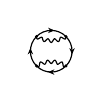
\begin{tikzpicture}[x=0.340cm, y=0.340cm, line width=0.420pt, baseline={([yshift=-0.6ex]0,0)}]
  \draw (-0.550,0.550) arc[start angle=135.000, end angle=45.000, radius=0.778];
  \fill (0.119,0.778) -- (-0.119,0.880) -- (-0.042,0.778) -- (-0.119,0.676) -- cycle;
  \draw plot[smooth, tension=0.7] coordinates {(0.550,0.550) (0.546,0.492) (0.526,0.459) (0.487,0.460) (0.437,0.489) (0.389,0.519) (0.353,0.526) (0.332,0.497) (0.317,0.442) (0.299,0.387) (0.271,0.360) (0.234,0.371) (0.192,0.411) (0.153,0.452) (0.120,0.467) (0.092,0.444) (0.064,0.395) (0.034,0.346) (0.000,0.326) (-0.034,0.346) (-0.064,0.395) (-0.092,0.444) (-0.120,0.467) (-0.153,0.452) (-0.192,0.411) (-0.234,0.371) (-0.271,0.360) (-0.299,0.387) (-0.317,0.442) (-0.332,0.497) (-0.353,0.526) (-0.389,0.519) (-0.437,0.489) (-0.487,0.460) (-0.526,0.459) (-0.546,0.492) (-0.550,0.550)};
  \draw (0.550,0.550) arc[start angle=45.000, end angle=-45.000, radius=0.778];
  \fill (0.778,-0.119) -- (0.880,0.119) -- (0.778,0.042) -- (0.676,0.119) -- cycle;
  \draw (-0.550,-0.550) arc[start angle=225.000, end angle=135.000, radius=0.778];
  \fill (-0.778,0.119) -- (-0.880,-0.119) -- (-0.778,-0.042) -- (-0.676,-0.119) -- cycle;
  \draw (0.550,-0.550) arc[start angle=315.000, end angle=225.000, radius=0.778];
  \fill (-0.119,-0.778) -- (0.119,-0.880) -- (0.042,-0.778) -- (0.119,-0.676) -- cycle;
  \draw plot[smooth, tension=0.7] coordinates {(0.550,-0.550) (0.499,-0.574) (0.463,-0.577) (0.445,-0.545) (0.437,-0.489) (0.426,-0.432) (0.402,-0.401) (0.363,-0.408) (0.317,-0.442) (0.273,-0.478) (0.239,-0.489) (0.213,-0.463) (0.192,-0.411) (0.168,-0.358) (0.137,-0.334) (0.101,-0.350) (0.064,-0.395) (0.031,-0.441) (0.000,-0.460) (-0.031,-0.441) (-0.064,-0.395) (-0.101,-0.350) (-0.137,-0.334) (-0.168,-0.358) (-0.192,-0.411) (-0.213,-0.463) (-0.239,-0.489) (-0.273,-0.478) (-0.317,-0.442) (-0.363,-0.408) (-0.402,-0.401) (-0.426,-0.432) (-0.437,-0.489) (-0.445,-0.545) (-0.463,-0.577) (-0.499,-0.574) (-0.550,-0.550)};
  \fill (0.550,0.550) circle (0.064);
  \fill (0.550,-0.550) circle (0.064);
  \fill (-0.550,0.550) circle (0.064);
  \fill (-0.550,-0.550) circle (0.064);
\end{tikzpicture}}
\diagramgap
\mbox{$\displaystyle -\,\frac{1}{4}$\,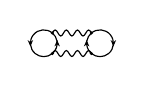
\begin{tikzpicture}[x=0.340cm, y=0.340cm, line width=0.420pt, baseline={([yshift=-0.6ex]0,0)}]
  \draw (-0.729,-0.383) arc[start angle=310.000, end angle=410.000, radius=0.500];
  \fill (-0.550,0.119) -- (-0.652,-0.119) -- (-0.550,-0.042) -- (-0.448,-0.119) -- cycle;
  \draw (-0.729,0.383) arc[start angle=50.000, end angle=310.000, radius=0.500];
  \fill (-1.550,-0.119) -- (-1.448,0.119) -- (-1.550,0.042) -- (-1.652,0.119) -- cycle;
  \draw (0.729,-0.383) arc[start angle=230.000, end angle=130.000, radius=0.500];
  \fill (0.550,0.119) -- (0.448,-0.119) -- (0.550,-0.042) -- (0.652,-0.119) -- cycle;
  \draw (0.729,0.383) arc[start angle=130.000, end angle=-130.000, radius=0.500];
  \fill (1.550,-0.119) -- (1.652,0.119) -- (1.550,0.042) -- (1.448,0.119) -- cycle;
  \draw plot[smooth, tension=0.7] coordinates {(-0.729,0.383) (-0.677,0.463) (-0.625,0.495) (-0.572,0.463) (-0.520,0.383) (-0.468,0.304) (-0.416,0.271) (-0.364,0.304) (-0.312,0.383) (-0.260,0.463) (-0.208,0.495) (-0.156,0.463) (-0.104,0.383) (-0.052,0.304) (0.000,0.271) (0.052,0.304) (0.104,0.383) (0.156,0.463) (0.208,0.495) (0.260,0.463) (0.312,0.383) (0.364,0.304) (0.416,0.271) (0.468,0.304) (0.520,0.383) (0.572,0.463) (0.625,0.495) (0.677,0.463) (0.729,0.383)};
  \draw plot[smooth, tension=0.7] coordinates {(-0.729,-0.383) (-0.677,-0.304) (-0.625,-0.271) (-0.572,-0.304) (-0.520,-0.383) (-0.468,-0.463) (-0.416,-0.495) (-0.364,-0.463) (-0.312,-0.383) (-0.260,-0.304) (-0.208,-0.271) (-0.156,-0.304) (-0.104,-0.383) (-0.052,-0.463) (0.000,-0.495) (0.052,-0.463) (0.104,-0.383) (0.156,-0.304) (0.208,-0.271) (0.260,-0.304) (0.312,-0.383) (0.364,-0.463) (0.416,-0.495) (0.468,-0.463) (0.520,-0.383) (0.572,-0.304) (0.625,-0.271) (0.677,-0.304) (0.729,-0.383)};
  \fill (-0.729,0.383) circle (0.064);
  \fill (-0.729,-0.383) circle (0.064);
  \fill (0.729,0.383) circle (0.064);
  \fill (0.729,-0.383) circle (0.064);
\end{tikzpicture}}
\diagramgap
\mbox{$\displaystyle +\,\frac{1}{2}$\,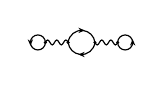
\begin{tikzpicture}[x=0.340cm, y=0.340cm, line width=0.420pt, baseline={([yshift=-0.6ex]0,0)}]
  \draw (0.500,0.000) arc[start angle=353.974, end angle=186.026, radius=0.503];
  \fill (-0.119,-0.450) -- (0.119,-0.552) -- (0.042,-0.450) -- (0.119,-0.348) -- cycle;
  \draw (-0.500,0.000) arc[start angle=173.974, end angle=6.026, radius=0.503];
  \fill (0.119,0.450) -- (-0.119,0.552) -- (-0.042,0.450) -- (-0.119,0.348) -- cycle;
  \draw plot[smooth, tension=0.7] coordinates {(-1.350,0.000) (-1.308,0.065) (-1.265,0.092) (-1.223,0.065) (-1.180,0.000) (-1.138,-0.065) (-1.095,-0.092) (-1.052,-0.065) (-1.010,0.000) (-0.968,0.065) (-0.925,0.092) (-0.883,0.065) (-0.840,0.000) (-0.798,-0.065) (-0.755,-0.092) (-0.712,-0.065) (-0.670,0.000) (-0.628,0.065) (-0.585,0.092) (-0.542,0.065) (-0.500,0.000)};
  \draw plot[smooth, tension=0.7] coordinates {(1.350,0.000) (1.308,-0.065) (1.265,-0.092) (1.223,-0.065) (1.180,0.000) (1.138,0.065) (1.095,0.092) (1.052,0.065) (1.010,0.000) (0.968,-0.065) (0.925,-0.092) (0.883,-0.065) (0.840,0.000) (0.798,0.065) (0.755,0.092) (0.712,0.065) (0.670,0.000) (0.628,-0.065) (0.585,-0.092) (0.542,-0.065) (0.500,0.000)};
  \draw (-1.350,0.000) arc[start angle=0.000, end angle=360.000, radius=0.280];
  \fill (-1.910,-0.119) -- (-1.808,0.119) -- (-1.910,0.042) -- (-2.012,0.119) -- cycle;
  \draw (1.350,0.000) arc[start angle=180.000, end angle=540.000, radius=0.280];
  \fill (1.910,0.119) -- (1.808,-0.119) -- (1.910,-0.042) -- (2.012,-0.119) -- cycle;
  \fill (-1.350,0.000) circle (0.064);
  \fill (1.350,0.000) circle (0.064);
  \fill (-0.500,0.000) circle (0.064);
  \fill (0.500,0.000) circle (0.064);
\end{tikzpicture}}
\diagramgap
\mbox{$\displaystyle -\,$\,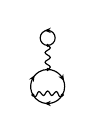
\begin{tikzpicture}[x=0.340cm, y=0.340cm, line width=0.420pt, baseline={([yshift=-0.6ex]0,0)}]
  \draw (-0.550,-0.318) arc[start angle=210.000, end angle=90.000, radius=0.635];
  \fill (-0.490,0.421) -- (-0.698,0.265) -- (-0.571,0.281) -- (-0.521,0.163) -- cycle;
  \draw (0.000,0.635) arc[start angle=90.000, end angle=-30.000, radius=0.635];
  \fill (0.610,0.214) -- (0.579,0.472) -- (0.529,0.354) -- (0.402,0.370) -- cycle;
  \draw (0.550,-0.318) arc[start angle=330.000, end angle=210.000, radius=0.635];
  \fill (-0.119,-0.635) -- (0.119,-0.737) -- (0.042,-0.635) -- (0.119,-0.533) -- cycle;
  \draw plot[smooth, tension=0.7] coordinates {(0.550,-0.318) (0.498,-0.365) (0.456,-0.380) (0.423,-0.349) (0.395,-0.285) (0.365,-0.220) (0.328,-0.190) (0.284,-0.209) (0.238,-0.263) (0.193,-0.317) (0.153,-0.338) (0.116,-0.311) (0.079,-0.251) (0.041,-0.192) (0.000,-0.168) (-0.041,-0.192) (-0.079,-0.251) (-0.116,-0.311) (-0.153,-0.338) (-0.193,-0.317) (-0.238,-0.263) (-0.284,-0.209) (-0.328,-0.190) (-0.365,-0.220) (-0.395,-0.285) (-0.423,-0.349) (-0.456,-0.380) (-0.498,-0.365) (-0.550,-0.318)};
  \draw plot[smooth, tension=0.7] coordinates {(0.000,1.535) (0.069,1.490) (0.097,1.445) (0.069,1.400) (0.000,1.355) (-0.069,1.310) (-0.097,1.265) (-0.069,1.220) (0.000,1.175) (0.069,1.130) (0.097,1.085) (0.069,1.040) (0.000,0.995) (-0.069,0.950) (-0.097,0.905) (-0.069,0.860) (0.000,0.815) (0.069,0.770) (0.097,0.725) (0.069,0.680) (0.000,0.635)};
  \draw (0.000,1.535) arc[start angle=270.000, end angle=630.000, radius=0.280];
  \fill (-0.119,2.095) -- (0.119,1.993) -- (0.042,2.095) -- (0.119,2.197) -- cycle;
  \fill (0.000,1.535) circle (0.064);
  \fill (0.000,0.635) circle (0.064);
  \fill (0.550,-0.318) circle (0.064);
  \fill (-0.550,-0.318) circle (0.064);
\end{tikzpicture}}
